\documentclass[10pt,a4paper]{article}
\usepackage[utf8]{inputenc}

% \usepackage{ngerman}  % german documents
\usepackage{graphicx}  % import graphics einbinden
\usepackage{listings}  % support source code listing
\usepackage{amsmath}  % math stuff
\usepackage{amssymb} % 
\usepackage{a4wide} % wide pages
\usepackage{fancyhdr} % nice headers
\usepackage{float}
\lstset{basicstyle=\footnotesize,language=Python,breaklines=true,numbers=left, numberstyle=\tiny, stepnumber=5,firstnumber=0, numbersep=5pt} % set up listings
\pagestyle{fancy}             % header
\setlength{\parindent}{0pt}   % no indentation

\usepackage[pdfpagemode=None, colorlinks=true,  % url coloring
           linkcolor=blue, urlcolor=blue, citecolor=blue, plainpages=false, 
           pdfpagelabels,unicode]{hyperref}
           
% change enums style: first level (a), (b), (c)           
\renewcommand{\labelenumi}{(\alph{enumi})}
\renewcommand{\labelenumii}{(\arabic{enumii})}

%lecture name
\newcommand{\lecture}{
	Bioinformatics III
}           

%assignment iteration
\newcommand{\assignment}{
	Second Assignment
}


%set up names, matricle number, and email
\newcommand{\authors}{
  \begin{tabular}{rl}
    \href{mailto:s8tbscho@stud.uni-saarland.de}{Thibault Schowing} & (2571837)\\
    \href{mailto:wiebkeschmitt@outlook.de}{Wiebke Schmitt} & (2543675)
  \end{tabular}
}

% use to start a new exercise
\newcommand{\exercise}[1]
{
  \stepcounter{subsection}
  \subsection*{Exercise \thesubsection: #1}

}

\begin{document}
\title{\Large \lecture \\ \textbf{\normalsize \assignment}}
\author{\authors}

\setlength \headheight{25pt}
\fancyhead[R]{\begin{tabular}{r}\lecture \\ \assignment \end{tabular}}
\fancyhead[L]{\authors}


\setcounter{section}{2} % modify for later sheets, i.e. 2, 3, ...
%\section{Introduction to Python and some Network Properties} % optional, note that section invocation sets the section counter + 1, so adapt the setcounter command
\maketitle

\exercise{The Scale-Free network}
\begin{enumerate}
	% A
\item \textit{Implement the algorithm given in the lecture to set up a scale-free network according to the
	Barabási-Albert model (see Lecture 2, slide 8). Start from the first three connected nodes
	and add each new node with a given number of links. Connect the new links with increasing
	preference to nodes that have higher degrees. This ScaleFreeNetwork-class should again
	use the abstract network class that you wrote in the first assignment.
	To obtain a much faster implementation and full points, think of a method to map the
	probabilities to connect to nodes somehow instead of computing them from scratch in each
	iteration.}\\

\textbf{Note:} We first generated the probability distribution in each iteration and use the function \textit{random.choices(pop, prob)} to select a node according to its probability (Method 1). After an intense reflection and the understanding of what what said during the tutorial, we tried a second option (Method 2) commented in the listing \ref{ex2-a}. The benchmark below (figure \ref{fig:timemethod2} and \ref{fig:timemethod1}) shows that the first option seems more time-efficient and thus we used this one to execute the program with the requested amount of nodes (100'000). 


\begin{figure}[H]
	\centering
	\label{fig:timemethod2}
	\caption{Time of execution with method 1 with 1000 and 10'000 nodes}
	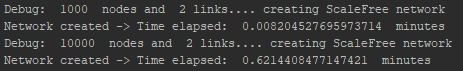
\includegraphics[width=0.7\linewidth]{img/time_method1}
	\label{fig:timemethod1}
	\caption{Time of execution with method 2 with 1000 and 10'000 nodes}
	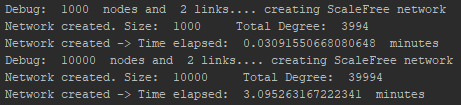
\includegraphics[width=0.7\linewidth]{img/time_method2}
\end{figure}


Implementation of the missing methods for the ScaleFreeNetwork-class. Listing \ref{ex2-a} shows source code of ScaleFreeNetwork.py and listing \ref{ex2-b} shows how the class has been tested.

\newpage
\lstinputlisting[label=ex2-a,caption={ScaleFreeNetwork.py}] {../Scripts/ScaleFreeNetwork.py}


% B
\item \textit{Determine the degree distributions for scale-free networks of 10 000 and 100 000 nodes
	(each with two new links per iteration), respectively, and plot them with double logarithmic
	axes. A new pre-implemented method in Tools.py will help you with that. What are the
	differences?
	Next, compare one of the distributions to the degree distribution of an equally sized random
	network (play around with the plot-scaling). What are the major differences?
}\\



%TODO img of scale vs scale -> img backup if fail with 100'000 and 10'000

\begin{figure}[H]
	\centering
	\includegraphics[width=0.7\linewidth]{"../Scripts/Plot_Degree Distribution of ScaleFree networks"}
	\caption{Two scale-free network, one with 10000 nodes and one with 100000 nodes. We can observe that the minimal probability depends highly on the network's size: the bigger the network, the lower the probability can go.}
	\label{fig:plotdegree-distribution-of-scalefree-networks}
\end{figure}


%TODO img of scale vs rand -> img backup if fail with 100'000
\begin{figure}[H]
	\centering
	\includegraphics[width=0.7\linewidth]{"../Scripts/Plot_Degree Distribution ScaleFree vs Random Network"}
	\caption[Scale-Free vs Random]{We can observe that the Scale-Free distribution follow a power-law style, as it is almost a straight line when plotted with log-log axes. On the other hand, the random network is more Poisson distributed as seen in Assignment 1.}
	\label{fig:plot2degree-distribution-scalefree-vs-random-network}
\end{figure}




% C
\newpage
\item \textit{The degree distribution of a scale-free network follows a power law, which has the form $P(k) ~ k^{-\lambda}$ To simplify the exercise, we assume $P(k) ~ Ck^{-\lambda}$ with $C$ being a fixed normalization
	constant to obtain a proper distribution. Try to fit this theoretical distribution to the
	degree distribution of a random network using the Kolmogorov-Smirnov distance. }\\


\lstinputlisting[label=ex2-b, caption={ScaleFreeTest.py}] {../Scripts/ScaleFreeTest.py}

\newpage
\lstinputlisting[label=ex2-c, caption={Tools.py}] {../Scripts/Tools.py}

\newpage
\textit{Use the KS distance to determine a $\gamma$ (between 1 and 3, 0.1 steps sufficient) that fits
	best to the degree distribution of a scale-free network with 10 000 nodes and two new
	links per iteration. Compare the empirical distribution of the network to the theoretical
	distribution with optimal $\gamma$ in a double-log. plot. Comment on the quality of your fit,
	reason why it may fail and how it could be vastly improved.}


%TODO discussion.... follows the theory until some point 
\begin{figure}[H]
	\centering
	\includegraphics[width=0.7\linewidth]{"../Scripts/Plot_Compare theory to practice"}
	\caption[Theory vs Practice]{ We can affirm that the scale-free distribution follows the power law at least asymptotically. For large values, the probability $P(k)$ for nodes having $ k $ connections to other nodes goes as $P(k) ~ k^{-\lambda}$. The only difference is speed at which the probability goes down when increasing the degree, as we can easily notice on the plot. To improve the fit, it would be a good idea to ignore the high degree nodes and fit the power law to the majority (fit the slope). }
	\label{fig:compare-theory-to-practice}
\end{figure}

\end{enumerate}


\newpage
\exercise{Classify real-world network examples}
\begin{enumerate}
	\item File sharing services\\
	
	 The two first listed services, Megaupload and Rapidshare, are more server oriented. The servers host the content, and the client download it. This is more like a scale-free network with a few big central servers around the world (so also like a clustered-network). About directions, each client can upload and download files (media like music and movies are certainly the most famous example). Of course, people uploading files are rarer than people downloading the contend. The traffic, so the directions, are more oriented from the hubs to the leaves/final client. 
	
	
	\item Social networks\\
	
	These are undirected networks. Two people are friends or not, but there is no directionality to
	the relation.
	A social network can be considered to be a scale-free network, because people with many
	friends are more likely to make new friends than people who are not as active socially. It can
	therefore also be considered to be a clustered network, because there tend to be people that
	are much more connected than others for geographical reasons. Celebrities can also form some kind of hub with many many connected people and form a local small-world. 
	
	
	\item Broadcasting networks\\
	
	This is hierarchical networks. Main TV/Radio companies send contents over cables or satellite connexion. For cables, city-relays, neighbourhood-relays or other structure can transmit the information stream from the central node, to the final one (TV or radio). The signal is directed from the broadcasting company to the client, so is the network.   
	

\end{enumerate}
	
	

\newpage
\exercise{Real interaction networks}
\begin{enumerate}
	\item Here is the implementation of the BioGRIDReader-class
	\lstinputlisting[label=ex23-c, caption={BioGRIDReader.py}] {../Scripts/BioGRIDReader.py}
	
	
	
	\newpage
	\item The class getMostAbundantTaxonIDs(n) is listed in the listing \ref{ex23-c} above. 
	
	\textbf{The most abundent TaxonIDs are (id, qty):  [('559292', 704012), ('9606', 414501), ('316407', 184023), ('284812', 72149), ('7227', 67935)]}
	
	\begin{itemize}
		\item 559292: Saccharomyces cerevisiae (Baker's Yeast)
		\item   9606: Human (Homo sapiens) 
		\item 316407: Escherichia coli
		\item 284812: Schizosaccharomyces pombe (Fission Yeast)
		\item   7227: Drosophila melanogaster
	\end{itemize}
	
	%todo why order not surprising
	The order is not surprising at all. All those organism are the most studied in history so it is not a surprise to find many results concerning them. 
	
	
	\item \textit{How big is the human interaction network and which are the 10 proteins with the highest
		degree? Take one of them as an example and briefly explain the biology behind the
		connectivity.}\\
	
	
	
	
	\textbf{Number of Human-Human interactions (human id = 9606):  386192}
	
	The  10  proteins with the highest degree are: 
	\textbf{[('TP53', 3024), ('TRIM25', 2559), ('APP', 2454), ('EGFR', 2134), ('UBC', 2042), ('NTRK1', 2002), ('MDM2', 1939), ('BRCA1', 1876), ('ELAVL1', 1840), ('HDAC1', 1646)]}\\
	
	
	The gene/protein P53 is the most present in the data. The protein's full name is "Cellular Tumor Antigen p53". "p53 has many mechanisms of anticancer function and plays a role in apoptosis, genomic stability, and inhibition of angiogenesis."\footnote{https://en.wikipedia.org/wiki/P53} This protein interacts with many cellular processes and thus, has many interactions with many other genes/proteins. 
	
	In our case, the human interaction network has \textbf{17087} nodes and \textbf{772384} links.
	
	
	\item Generic network distribution and implementation 
	
	
\begin{figure}[H]
	\centering
	\includegraphics[width=0.7\linewidth]{"../Scripts/Plot_Degree Distribution Generic Network "}
	\caption[Human interaction network plot]{Human interaction degree distribution}
	\label{fig:plot4degree-distribution-generic-network-}
\end{figure}
	
	We can observe that there is indeed a mix between the scale free straight slope and flat probability as it reaches big degrees and the slight curvature as if it was mixed with a bell-curve distribution. Of course, this is closer to a scale free network. Important molecules/proteins play a role in many reaction and more complex ones might have only a few purposes. The bump on the line is the small part of randomness in the nature that makes it different from maths. \\
	
	\lstinputlisting[label=ex23-d, caption={GenericNetwork.py}] {../Scripts/GenericNetwork.py}
	
	
	
\end{enumerate}	
	




\end{document}